\chapter{LUI Gesture Elicitation Studies} \label{app:lui-ges}


%===================================================================================
\section{Photo- and Video-Browsing Gesture Elicitation Studies}
\label{app:lui-ges:initial}
Two experiments were conducted to determine users' preferred gestures for browsing photos and videos. 30 participants (16 female) aged between 18 and 77 years old ($M{=}34.5$, $SD{=}17.5$) took part in the photo-browsing experiment while 22 participants (8 females) aged between 15 and 54 years old ($M{=}28.9$, $SD{=}12.6$) took part in the video-browsing experiment. Agreement rates ranged from .064 to .690 ($M{=}.205$, $SD{=}.147$) in the photo-browsing experiment (\tab~\ref{tbl:lui-ges:agreement-photo}) and from .052 to .593 ($M{=}.229$, $SD{=}.162$) in the video-browsing experiment (\tab~\ref{tbl:lui-ges:agreement-video}).

\begin{table*}[ht]
	% \resizebox{\linewidth}{!}{
	\renewcommand{\arraystretch}{1.1}
	\captionsetup{justification=centering}
	\footnotesize
	\begin{tabular}{p{3.35cm}rp{2.875cm}p{2.975cm}}
		\toprule
		\textbf{Referent} & \multicolumn{1}{l}{\textbf{AR}} & \textbf{1\textsuperscript{st} most agreed gesture} & \textbf{2\textsuperscript{nd} most agreed gesture} \\
		\midrule
		1. \textit{Pan photo gallery right} & \cellcolor{highlightcolor} .251 (M) & 1 hand flick & Multiple fingers swipe\\
        2. \textit{Pan photo gallery left} & \cellcolor{highlightcolor} .269 (M) & Multiple fingers swipe & 1 finger swipe\\
        3. \textit{Pan photo gallery up} & .170 (M) & 1 finger swipe & Hand rotation\\
        4. \textit{Pan photo gallery down} & .175 (M) & 1 hand flick & 1 finger swipe\\
        5. \textit{Go to next page of photo gallery} & .205 (M) & Multiple fingers swipe & 1 hand flick\\
        6. \textit{Go to previous page of photo gallery} & .168 (M) & Multiple fingers swipe & 1 hand flick\\
        7. \textit{Zoom in a photo} & \cellcolor{highlightcolor} .338 (H) & Splay the hand & Move hands apart\\
        8. \textit{Zoom out a photo} & \cellcolor{highlightcolor} .299 (M) & Clench the hand & Move hands apart\\
        9. \textit{Maximize a photo from normal view to full screen} & \cellcolor{highlightcolor} .363 (H) & Move hands apart & Splay the hand\\
        10. \textit{Unmaximize a photo from full screen to normal view} & .193 (M) & Clench the hand & Move hands closer together\\
        11. \textit{Open photo information} & \cellcolor{highlightcolor} .308 (H) & 1 finger tap & Splay the hand\\
        12. \textit{Close photo information} & .170 (M) & 1 finger tap & 1 finger swipe\\
        13. \textit{Set layout to carousel} & .099 (L) & Hand rotation & 1 finger tap\\
        14. \textit{Start slideshow} & .126 (M) & 1 finger tap & Hand pose\\
        15. \textit{Stop slideshow} & .156 (M) & 1 finger tap & Move flat hand forward/backward\\
        16. \textit{Take a selfie} & .099 (L) & Hand pose & 1 finger tap\\
        17. \textit{Insert a new photo} & .092 (L) & Hand pose & 1 finger tap\\
        18. \textit{Duplicate a photo} & .097 (L) & 1 finger swipe & 1 finger tap\\
        19. \textit{Delete a photo} & .094 (L) & 1 finger swipe & Hand pose\\
        20. \textit{Crop a photo} & .090 (L) & Draw & Move hands apart\\
        21. \textit{Resize a photo} & \cellcolor{highlightcolor} .333 (H) & Move hands apart & Splay the hand\\
        22. \textit{Rotate a photo 90\textdegree CW} & \cellcolor{highlightcolor} .634 (V) & Hand rotation & N/A\\
        23. \textit{Rotate a photo 90\textdegree CCW} & \cellcolor{highlightcolor} .690 (V) & Hand rotation & N/A\\
        24. \textit{Increase constrast} & .071 (L) & 1 finger swipe & Open arms (with flat hands)\\
        25. \textit{Decrease contrast} & .064 (L) & 1 finger swipe & Multiple fingers swipe\\
        26. \textit{Dock a photo} & .097 (L) & 1 finger swipe & 1 hand flick\\
        27. \textit{Undock a photo} & .152 (M) & 1 finger swipe & Take and throw\\
        28. \textit{Like a photo} & \cellcolor{highlightcolor} .218 (M) & 1 finger tap & Hand pose\\
        29. \textit{Search by criteria} & .131 (M) & Hand pose & Draw\\
        30. \textit{Share a photo with somebody (vocal email)} & .087 (L) & Hand pose & 1 finger swipe\\
        31. \textit{Convert a photo into another format} & .115  (M) & Move hands apart & 1 finger tap\\
		\bottomrule
	\end{tabular}
	% }
	\caption{First and second most agreed gesture proposals for each referent (photo-browsing experiment). Referents with above-average agreement rates are highlighted in blue. Notation for the Agreement Rate (AR): L${=}$low, M${=}$medium, H${=}$high, V${=}$very high~\cite{Vatavu:2015}.}
	\label{tbl:lui-ges:agreement-photo}
	\vspace{-10pt}
\end{table*}

\begin{table*}[ht]
    % \resizebox{\linewidth}{!}{
	\renewcommand{\arraystretch}{1.1}
	\captionsetup{justification=centering}
	\footnotesize
	\begin{tabular}{p{3.35cm}rp{2.875cm}p{2.975cm}}
		\toprule
		\textbf{Referent} & \multicolumn{1}{c}{\textbf{AR}} & \textbf{1\textsuperscript{st} most agreed gesture} & \textbf{2\textsuperscript{nd} most agreed gesture} \\
		\midrule
		1. \textit{Pan video gallery right} & \cellcolor{highlightcolor} .433 (H) & 1 hand drag & 1 finger drag\\
        2. \textit{Pan video gallery left} & \cellcolor{highlightcolor} .433 (H) & 1 hand drag & 1 finger drag\\
        3. \textit{Pan video gallery up} & \cellcolor{highlightcolor} .390 (H) & 1 hand drag & 1 finger drag\\
        4. \textit{Pan video gallery down} & \cellcolor{highlightcolor} .390 (H) & 1 hand drag & 1 finger drag\\
        5. \textit{Go to next page of video gallery} & \cellcolor{highlightcolor} .407 (H) & 1 hand drag & 1 finger drag\\
        6. \textit{Go to previous page of video gallery} & \cellcolor{highlightcolor} .329 (H) & 1 hand drag & 1 finger drag\\
        7. \textit{Zoom in a video} & .182 (M) & 1 hand drag & Close one hand\\
        8. \textit{Zoom out a video} & \cellcolor{highlightcolor} .242 (M) & 1 hand drag & Close one hand\\
        9. \textit{Set a video in full screen} & .165 (M) & 1 finger tap & Drag 1 finger from each hand\\
        10. \textit{Unmaximize a video from full screen to normal view} & .095 (L) & Drag 1 finger from each hand & 2 hands drag\\
        11. \textit{Play a video} & \cellcolor{highlightcolor} .333 (H) & 1 finger tap & 1 finger drag\\
        12. \textit{Stop playing a video} & \cellcolor{highlightcolor} .294 (M) & Push/pull 1 hand & 1 finger tap\\
        13. \textit{Move to the beginning of video} & .169 (M) & 1 hand drag & 1 finger tap\\
        14. \textit{Move to the end of a video} & .169 (M) & 1 hand drag & 1 finger tap\\
        15. \textit{Open video information} & .117 (M) & 1 finger tap & Push/pull 1 hand\\
        16. \textit{Close video information} & .117 (M) & 1 hand drag & 1 finger drag\\
        17. \textit{Set layout to carousel} & .117 (M) & 1 hand drag & Tap and drag 1 finger\\
        18. \textit{Insert a new video} & .078 (L) & Push/pull and drag 1 hand & Push/pull 1 hand\\
        19. \textit{Duplicate a video} & .052 (L) & 2 hands drag & Tap and drag 1 finger from each hand\\
        20. \textit{Delete a video} & .074 (L) & 1 hand drag & 1 finger drag\\
        21. \textit{Rotate a video 90\textdegree CW} & \cellcolor{highlightcolor} .593 (V) & 1 hand drag & Push/pull 1 hand\\
        22. \textit{Rotate a video 90\textdegree CCW} & \cellcolor{highlightcolor} .593 (V) & 1 hand drag & Push/pull 1 hand\\
        23. \textit{Dock a video} & .078 (L) & Push/pull and drag 1 hand & Tap and drag 1 finger\\
        24. \textit{Undock a video} & .078 (L) & Push/pull and drag 1 hand & Close, push/pull and drag 1 hand\\
        25. \textit{Like a video} & .091 (L) & 1 finger drag & Push/pull 1 hand\\
        26. \textit{Search for a video by criteria} & .082 (L) & 1 finger drag & 1 hand drag\\
        27. \textit{Share a video with somebody} & .082 (L) & 1 hand drag & Close, push/pull and drag 1 hand\\
		\bottomrule
	\end{tabular}
	% }
	\caption{First and second most agreed gesture proposals for each referent (video-browsing experiment). Referents with above-average agreement rates are highlighted in blue. Notation for the Agreement Rate (AR): L${=}$low, M${=}$medium, H${=}$high, V${=}$very high~\cite{Vatavu:2015}.}
	\label{tbl:lui-ges:agreement-video}
	% \vspace{-10pt}
\end{table*}


%===================================================================================
\section{Multimedia Gesture Elicitation Study} \label{app:lui-ges:new}
A third GES was conducted to elicit mid-air gestures for multimedia interaction (Section~\ref{sec:lui:development-method:gesture-set}). Section~\ref{app:lui-ges:protocol} provides details about the experimental protocol and Section~\ref{app:lui-ges:results} presents its results.

%\subsection{Experiment}
%\label{app:elicitation:experiment}
%The experiment was initially performed to elicit both mid-air and touch gestures for interacting with multimedia content such as photos and videos. However, only the mid-air gesture proposals are discussed here as touch gestures are not relevant for this specific application.
%\noindent
\subsection{Experimental Protocol} \label{app:lui-ges:protocol}
\subsubsection{Participants} 
23 participants (6 females), aged from 18 to 56 years old ($M{=} 27.1$, $SD{=}10.2$ years), volunteered for the study. Their occupations include students and employees, mostly in IT, art, and engineering. All but two of the participants never used an LMC, but all of them regularly used a computer. Only one participant did not frequently use a smartphone. 95.7\% of the participants (22/23) were right-handed.


\begin{figure}[h!]
    \centering
    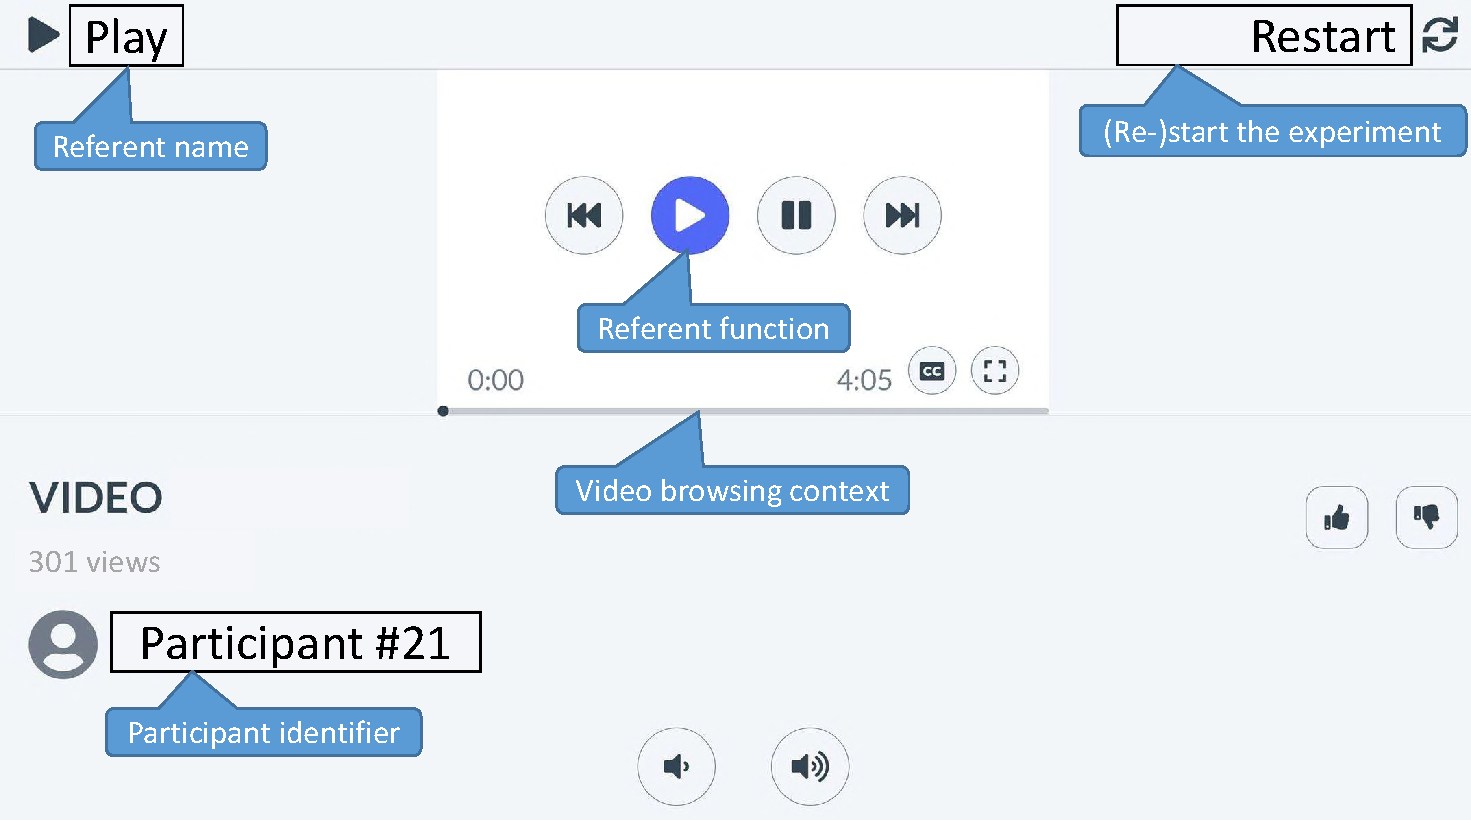
\includegraphics[width=\textwidth]{Figures/App-LUIGES/ges-ui.pdf}
    % \vspace{-8pt}
    \caption{Screenshot of the gesture elicitation software.}
    \label{fig:lui-ges:real}
    % \vspace{-6pt}
\end{figure}

\subsubsection{Apparatus}
The experiment involved three devices: the LMC to capture participants' mid-air gesture proposals, a smartphone to record their touch gesture proposals, and a large screen to display the referents. %A laptop computer was used to control the display and record the gestures captured by the LMC using custom software for contextual gesture elicitation\footnote{We release its code on GitHub at \url{https://github.com/anonymous/recorder}}. This application presents functions (see \tab~\ref{tab:media-actions}) depending on the media randomly selected and enables participants to record their gesture one or multiple times (Fig.~\ref{fig:contextual}).
A laptop controlled the display and recorded the LMC gestures using custom software suited for gesture elicitation~\ref{fig:lui-ges:real}.
%\footnote{We release its code on GitHub at \url{https://github.com/anonymous/elicitation} and \url{https://github.com/anonymous/recorder}}. The software presents functions (see \tab~\ref{tab:media-actions}) depending on the media randomly selected (Fig.~\ref{fig:real}) and enables participants to record their gestures.
% TODO


\subsubsection{Design} 
The experiment manipulates one main independent variable:
\textsc{Referent}, a within-subject nominal variable with 18 conditions. Each condition represents a common task to perform in multimedia environments, such as in a music player, a video gallery, or a PowerPoint presentation: (1) previous, (2) next, (3) enable fullscreen, (4) disable fullscreen, (5) zoom in, (6) zoom out, (7) volume up, (8) volume down, (9) rotate 90\textdegree clockwise, (10) rotate 90\textdegree counter-clockwise, (11) play, (12) pause, (13) like, (14) dislike, (15) fast forward 5 seconds, (16) rewind 5 seconds, (17) enable subtitles, and (18) disable subtitles. The number of conditions has been purposefully kept small by combining similar referents for different contexts together, \eg there is no distinction between going to the next picture and going to the next video.

The following measures were employed to evaluate and understand users' preferences for gestures captured by the LMC~\cite{Gheran:2018}:
\begin{enumerate}[noitemsep]
    \item The agreement rate $AR(r)$ was computed for each \textsc{Referent}.% using the formula of ~\cite{Vatavu:2015}
    %, as follows:
    %\vspace{-4pt}
%   \begin{equation}
%       AR(r) = \frac{\sum_{i<j}{\delta_{i,j}}}{n \cdot (n-1) / 2}
%           \vspace{-4pt}
%   \end{equation}
%   where $n$ is the number of participants from which gestures are elicited, and $\delta_{i,j}$ evaluates to $1$ if the $i$-th and $j$-th participants are in agreement over referent $r$ and to $0$ otherwise. 

    \item The \textsc{Thinking-Time} measures the time, in seconds, needed by participants to propose a gesture for a given referent.
    
    \item The \textsc{Goodness-of-Fit} represents participants' subjective assessment, as a rating between 1 and 5, of their confidence about how well a gesture fits a referent.
\end{enumerate}

%     \item \textsc{Interaction method}: a within-subject nominal variable with 2 conditions: (1) touch gesture, and (2) mid-air gesture. Only the participants' mid-air gesture propositions are relevant to this paper.
    
%     \item \textsc{Proposition sequence}, a between-subject nominal variable with 2 conditions: (1) for each referent, the participant first proposes a touch gesture and then a mid-air gesture, and (2) for each referent, the participant first proposes a mid-air gesture and then a touch gesture.
% \end{itemize}

%\vspace{-16pt}
\subsubsection{Task}
Participants were installed at a desk and faced a large screen situated a few meters on the opposite side of the desk. The LMC was positioned in front of them, and a smartphone was placed on their right. Each participant was presented with a series of referents in a randomized order. For each referent, participants were asked to propose a mid-air gesture that fits the referent, in an order determined randomly. Participants' thinking time was measured for each gesture proposal. No constraint was imposed on the participants' choices. After each gesture proposal, the participants estimated its goodness-of-fit on a Likert scale from 1 (very unsatisfied) to 5 (very satisfied).


%===================================================================================


\subsection{Results} \label{app:lui-ges:results}
414 mid-air gesture proposals were collected from 23 (participants) $\times$ 18 (referents) conditions. These gesture proposals were then clustered into 112 groups of similar gestures. For this clustering, we distinguished between gestures according to their direction (\ie similar gestures performed in different directions are considered different) but grouped similar gestures performed with different poses together (\eg swiping with a flat hand is considered the same as swiping while pointing the index finger). \tab~\ref{tbl:lui-ges:gesture-proposals} summarizes the most agreed-upon gestures for each referent.

\begin{table*}[ht]
    % \resizebox{\linewidth}{!}{
    \footnotesize
    \renewcommand{\arraystretch}{1.1}
    \begin{tabular}{p{3.35cm}rp{2.875cm}p{2.975cm}}
        \toprule
        \textbf{Referent} & \multicolumn{1}{c}{\textbf{AR}} & \textbf{1\textsuperscript{st} most agreed gesture} & \textbf{2\textsuperscript{nd} most agreed gesture} \\
        \midrule
        1. \textit{Previous} & \cellcolor{highlightcolor}.498 (H) & Flick right & Flick left \\
        2. \textit{Next} & \cellcolor{highlightcolor}.498 (H) & Flick left & Flick right \\
        3. \textit{Enable fullscreen} & .273 (M) & Move hands apart & Pinch out \\
        4. \textit{Disable fullscreen} & .146 (M) & Move hands closer together & Pinch in \\
        5. \textit{Zoom in} & .320 (H) & Pinch out & Move hands apart \\
        6. \textit{Zoom out} & .300 (M) & Pinch in & Move hands closer together \\
        7. \textit{Volume up} & \cellcolor{highlightcolor} .478 (H) & Swipe up & Rotate a knob CW \\
        8. \textit{Volume down} & .316 (H) & Swipe down & Rotate a knob CCW \\
        9. \textit{Rotate 90\textdegree CW} & \cellcolor{highlightcolor} .830 (V) & Rotate a knob CW & N/A \\
        10. \textit{Rotate 90\textdegree CCW} & \cellcolor{highlightcolor} .830 (V) & Rotate a knob CCW & N/A \\
        11. \textit{Play} & .190 (M) & Tap with the index finger & Draw the ``play'' symbol \\
        12. \textit{Pause} & .166 (M) & Tap with the index finger & Swipe down with two fingers \\
        13. \textit{Like} & \cellcolor{highlightcolor} .751 (V) & Thumb up & N/A \\
        14. \textit{Dislike} & \cellcolor{highlightcolor} .751 (V) & Thumbs down & N/A \\
        15. \textit{Fast-forward 5 seconds} & .087 (L) & Flick right twice & Swipe left \\
        16. \textit{Rewind 5 seconds} & .095 (L) & Swipe right & Flick left twice \\
        17. \textit{Enable subtitles} & .032 (L) & Swipe up & Push \\
        18. \textit{Disable subtitles} & .028 (L) & Swipe down & Pull \\
        \bottomrule
    \end{tabular}
    % }
    \caption{First and second most agreed gesture proposals for each referent. Referents with above-average agreement rates are highlighted. Magnitude of the Agreement Rate ($AR$)~\cite{Vatavu:2015}: L${=}$low, M${=}$medium, H${=}$high, V${=}$very high.}
    \label{tbl:lui-ges:gesture-proposals}
    \vspace{-8pt}
\end{table*}

\subsubsection{Consensus}
Overall, agreement rates are quite high, between .028 and .83 ($M{=}.366$, $SD{=}.268$). These results fit within the reported agreement rates in the literature of gesture elicitation, see \cite{Vatavu:2015} (\mbox{p. 1332}) that summarize agreement rates of 18 studies. According to the recommendations of ~\cite{Vatavu:2015} to interpret the magnitudes of agreement rates, most of our results fall inside the high consensus (.300$-$.500) category. These results were confirmed by Kendall's coefficient of concordance for estimating the inter-rater reliability: $W{=}.564$ ($\chi^2(26){=}220.454$, $p{<}.0001$, large effect).

\subsubsection{Gestures' Goodness of Fit}
Participants rated their gesture proposals with numbers from 1 (poor fit) to 5 (excellent fit) to denote their confidence in the goodness of fit of their proposals. Overall, participants were satisfied with their gesture propositions as shown by the high average goodness of fit ($M{=}4.21$, $SD{=}0.88$).
\textsc{Goodness-of-Fit} correlated significantly with the \textsc{Agreement-Rate} (Pearson's $r_{(N{=}18)}{=}.711$, $R^2{=}.505$, $p{=}.00094$): referents that reached high agreement rates were assigned gestures that were rated a good fit (\fig~\ref{fig:goodness-of-fit}).

\begin{sidewaysfigure}[ht]
    \centering
    \captionsetup{justification=centering}
    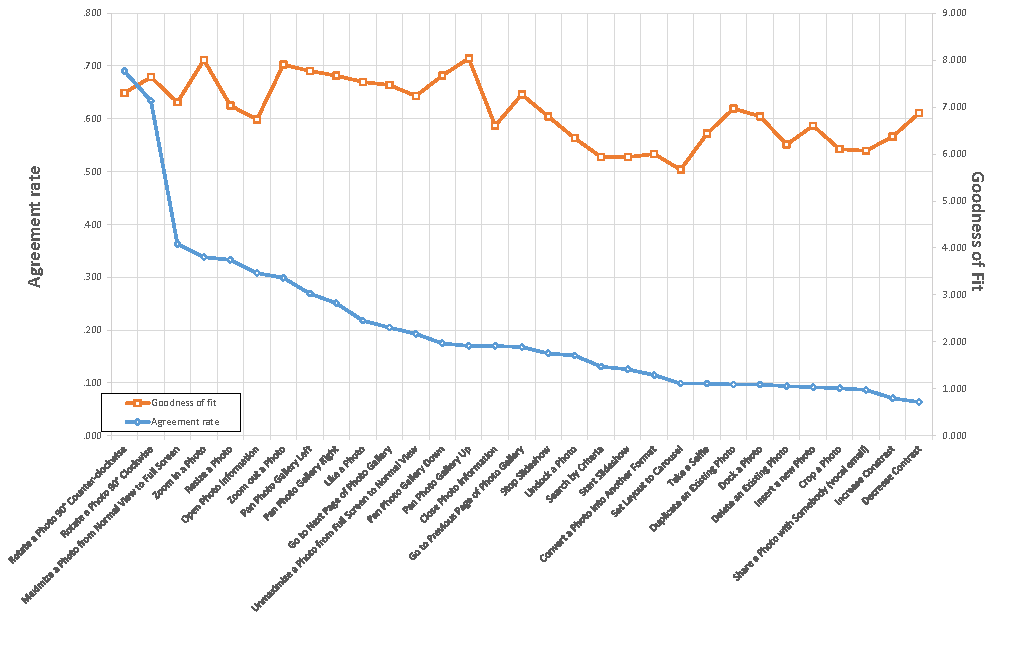
\includegraphics[width=.99\linewidth]{Figures/App-LUIGES/goodness-of-fit.pdf}
    % \vspace{-24pt}
    \caption{Relationship between \textsc{Agreement-Rate} and \textsc{Goodness-of-Fit}.}
    \label{fig:goodness-of-fit}
    % \vspace{-8pt}
\end{sidewaysfigure}

\subsubsection{Thinking Time}
The average thinking time was usually quite low ($M{=}6.15$\,s, $SD{=}9.12$\,s). 
\textsc{Thinking-Time} correlated significantly with \textsc{Agreement-Rate} (Pearson's $r_{(N=18)}{=}-.620$, $R^2{=}.384$, $p{=}.006$) (Fig.~\ref{fig:thinking-time}): the agreement rate decreased for longer thinking times. A few referents showed considerably higher than average thinking times: disable subtitles, enable subtitles, and skip backward 5 seconds. These referents represent tasks that participants are less likely to perform regularly on their devices.

\begin{sidewaysfigure}[ht]
    \centering
    \captionsetup{justification=centering}
    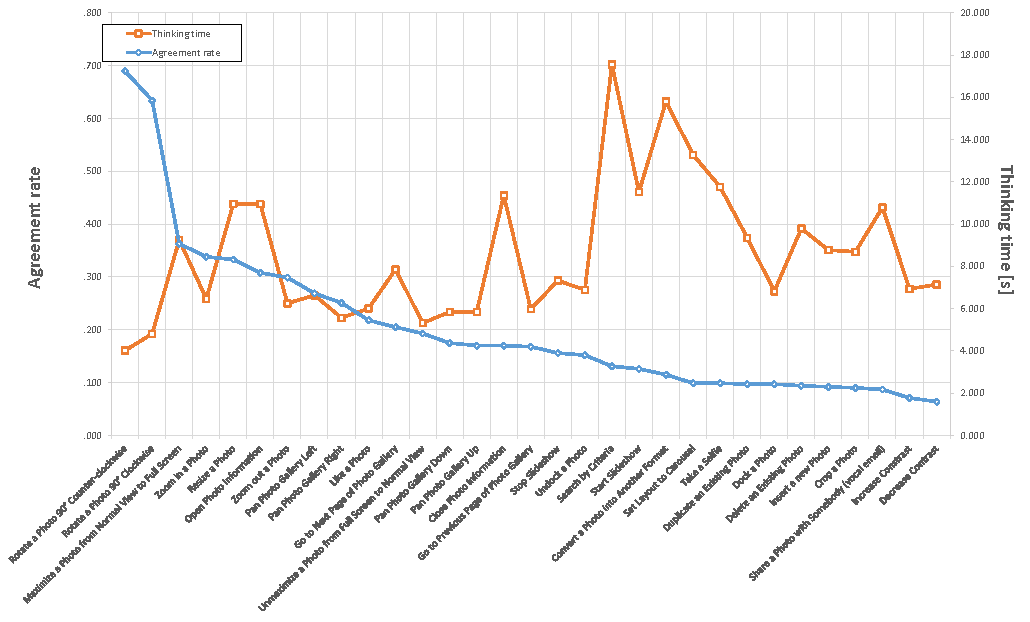
\includegraphics[width=\linewidth]{Figures/App-LUIGES/thinking-time.pdf}
    % \vspace{-15pt}
    \caption{Relationship between \textsc{Agreement-Rate} and \textsc{Thinking-Time}.}
    \label{fig:thinking-time}
    % \vspace{-8pt}
\end{sidewaysfigure}




